\documentclass[a4paper,11pt]{article}

% set up sensible margins (same as for cssethesis)
\usepackage[paper=a4paper,left=30mm,right=30mm,top=25mm,bottom=25mm]{geometry}
\usepackage{natbib} % Use the natbib bibliography and citation package
\usepackage{setspace} % This is used in the title page
\usepackage{graphicx} % This is used to load the crest in the title page
\usepackage{physics} % Used for \abs

% non-template packages
\usepackage{paralist}
\usepackage{multicol}
\usepackage{caption}
\usepackage{tabularx, booktabs}
\newcolumntype{Y}{>{\centering\arraybackslash}X}
\usepackage{listings}
\lstset{
	numbers=left, 
	numberstyle=\small, 
	numbersep=8pt, 
	frame = single, 
	language=Python, 
	framexleftmargin=17pt}

\usepackage{tikz}
\usepackage{smartdiagram}

\usepackage[font={small,it}]{caption}
\usepackage{hyperref}
\usepackage{xcolor}
\usepackage{lscape}
\hypersetup{
	colorlinks,
	linkcolor=teal,
	citecolor=teal,
	urlcolor=blue
}

\usepackage[english]{babel}
\usepackage{blindtext}
\usepackage{footnote}
\makesavenoteenv{tabular}
\makesavenoteenv{table}

%tikz stuff
\usepackage{tikz}
\usetikzlibrary{shapes, arrows, trees}
\tikzstyle{decision} = [diamond, draw, fill=green!20, text width=4.5em, text badly centered, node distance=3cm, inner sep=0pt]
\tikzstyle{block} = [rectangle, draw, fill=yellow!20, text width=3cm, text centered, rounded corners, minimum height=4em]
\tikzstyle{line} = [draw, -latex']
\tikzstyle{straight} = [draw]


\usepackage{array}
\newcolumntype{L}[1]{>{\raggedright\let\newline\\\arraybackslash\hspace{0pt}}m{#1}}
\newcolumntype{C}[1]{>{\centering\let\newline\\\arraybackslash\hspace{0pt}}m{#1}}
\newcolumntype{R}[1]{>{\raggedleft\let\newline\\\arraybackslash\hspace{0pt}}m{#1}}

\usepackage{float}

\usepackage{amsmath}
\usepackage{algorithm}
\usepackage{algorithmicx}
\usepackage[noend]{algpseudocode}

\floatname{algorithm}{Procedure}
\renewcommand{\algorithmicrequire}{\textbf{Input:}}
\renewcommand{\algorithmicensure}{\textbf{Output:}}

\algdef{SE}[DOWHILE]{DoWhile}{EndDoWhile}{\algorithmicdo}[1]{\algorithmicwhile\ #1}%
\algdef{SE}[DOWHILE]{Do}{EndDo}{\algorithmicdo}[1]{#1}

\newcommand{\Break}{\State\textbf{break}}

\let\oldReturn\Return
\renewcommand{\Return}{\State\oldReturn}

\usepackage{colortbl}

%\hypersetup{
%	colorlinks,
%	linkcolor={red!50!black},
%	citecolor={blue!50!black},
%	urlcolor={blue!80!black}
%}

\begin{document}
	
% Set up a title page
\thispagestyle{empty} % no page number on very first page
% Use roman numerals for page numbers initially
\renewcommand{\thepage}{\roman{page}}

\begin{spacing}{1.5}
	\begin{center}
		{\Large \bfseries
			School of Computer Science (BICA) \\
			Monash University}
		
		
		\vspace*{30mm}
		
		
\includegraphics[width=5cm]{graphics/MonashCrest.pdf}
		
		\vspace*{15mm}
		
		{\large \bfseries
			Literature Review, 2017
		}
		
		\vspace*{10mm}
		
		{\LARGE \bfseries
			Review of optimal multi-agent Pathfinding algorithms and usage in warehouse automation
		}
		
		\vspace*{20mm}
		
		{\large \bfseries
			Phillip Wong
			
			\vspace*{20mm}
			
			
			Supervisors: \parbox[t]{50mm}{Daniel Harabor,\\Pierre Le Bodic}
		}
		
	\end{center}
\end{spacing}

\newpage

\tableofcontents

\newpage
% Now reset page number counter,and switch to arabic numerals for remaining
% page numbers 
\setcounter{page}{1}
\renewcommand{\thepage}{\arabic{page}}

\section{Introduction} \label{sec:introduction}

In our multi-agent pathfinding problem, we have an environment containing a set of $k$ agents on a 4 directional grid-map. Each agent aims to find a path to their goal such that no agent will collide with another agent at any time.

Hence we have a centralized agent coordinator which aims to resolve path collisions.

\subsection{Problem Overview}
\noindent \textbf{Inputs:}
\begin{itemize}
	\item Grid map
	\item Set of agents with
	\begin{itemize}
		\item Start location
		\item Goal location
	\end{itemize}
\end{itemize}

\noindent \textbf{Outputs:}
\begin{itemize}
	\item Collision free path from the start to goal location for each each agent
\end{itemize}

\begin{Large}
	INSERT IMAGE OF EXAMPLE PROBLEM
\end{Large}



\subsection{Use of Mixed Integer Programming}
\noindent \textbf{Branch and bound}

\noindent \textbf{Column generation}

\noindent \textbf{Branch and price}

\section{Related Work}
\textbf{CBS}

\textbf{ICTS}

\textbf{Centralised A*}

\textbf{That Network Flow paper}

\section{Algorithm}
Each agent knows of a number of paths to the goal. Using a Mixed Integer Program (MIP) we are able to solve the assignment problem of choosing a combination of paths such that no assigned two paths has a collision. Hence the two main parts of the algorithm:

Any specifics about the MIP I should mention here? 

\begin{compactenum}
	\item \textbf{Path Assignment} The Mixed Integer Program, Responsible for choosing a assigning paths to agents, while finding a conflict-free solution.
	\item \textbf{Path Generation:} Responsible for generating alternative paths for agents whose current paths are in collision.
\end{compactenum}

\subsection{High Level Description} \label{sec:high-level}
At the high-level we describe the cycle of path generation and assignment. 

\noindent \textbf{Initializing:} Starting on line \ref{pathbank}, we find the shortest path to each agent's goal and add it to their path bank. A path bank is simply a pool of valid paths to each agent's goal, these paths can be non-optimal.

\noindent \textbf{Calling the MIP:} Starting the loop, we call AssignPathsMIP. Here we create and run the Mixed Integer Program. This method will choose suitable paths from each agent's path pool. Importantly we have not yet described the second parameter, pathCollisions. Hence we do not know if the assignment is collision-free. 

\noindent \textbf{Checking collisions:} So we must check if the solution the MIP gave us is valid.

\noindent \textbf{No collision?:} If there was no collision, then the solution the MIP assigned us was valid and we can terminate the algorithm.

\noindent \textbf{Collision occured:} If there was a collision, we must perform extra steps. The goal here is to penalize this collision and generate new alternative paths. Hence we add this collision to the pathCollisions (used in the AssignPathMIP method), this later creates a hard constraint saying path $i$ for agent $n$ and path $j$ for agent $m$ cannot exist at the same time. Hence the MIP will not be able to choose these two in combination.

\noindent \textbf{Choosing an agent:} This method deals with choosing the next agent who we generate a path for. Here we choose the agent with the smallest $\Delta$. This value describes the length between the shortest path and the current path. By choosing the agent with the smallest $\Delta$ we can ensure optimality as the makespan of the solution grows incrementally \textit{IMPORTANT: describe this better}.

\noindent \textbf{Penalties:} Now we penalize the collision. We do this by looking at the perspective of the chosen agent. So for a collision between $a_np_i$ and $a_mp_j$, say we have chosen $a_n$. Hence we are interested in penalizing against $p_j$. The penalty applies a negative value to any action that could lead to a collision against $p_j$ \textbf{EXAMPLE HERE OR LINK TO EXAMPLE?}.

\noindent \textbf{Looping:} Now we repeat this iteration of assignment and applying penalties. By ensuring that the makespan of the solution space grows incrementally by 1. We can generate an optimal solution, as the MIP will find a possible combination of paths from each agent's path bank.

\begin{algorithm}[H]
	\begin{algorithmic}[1]
		\Require $agents:$ list of agents
		\Ensure an assignment of collision-free paths
		\State{find and store shortest path for each agent}
		\Loop
			\State{run the MIP and apply the path assignment solution}
			\State{check the path assignment for collisions}
			\If{there are no collisions}
				\Return current path assignments
			\Else
				\State{get the path collision with the lowest $\Delta$}
				\State{for the two agents in this collision: find and store an alternative path}
				\State{create path constraints from this path collision and apply to the MIP}
			\EndIf
		\EndLoop
	\end{algorithmic}
	
	\caption{high-level algorithm} \label{alg:agent-coordinator}
\end{algorithm}

\begin{algorithm}[H]
	\begin{algorithmic}[1]
		\Require $agents:$ list of agents
		\Ensure $void$
		\State{$pathCollisions \gets \{\}$}
		\State{$penalties \gets Map<Agent, Penalties>()$}
		\State{}
		\For{$agent : agents$}
			\State{$agent.pathBank.add(ShortestPath(agent))$}
		\EndFor
		\State{}
		\Loop
			\State{$assignedPaths \gets AssignPathsMIP(agents, pathCollisions)$}
			\State{$collision \gets CheckForACollision(assignedPaths)$}
			\If{\textit{collision is not none}}
				\State{$pathCollisions.add(collision)$}
				\State{$chosenAgent \gets ChooseAgent(collision)$}
				\State{$UpdatePenalties(chosenAgent)$}
				\State{$chosenAgent.pathBank.add(GenerateNextBestPath(agent, penalties))$}
			\Else
				\Break
			\EndIf
		\EndLoop
	\end{algorithmic}
	
	\caption{high-level algorithm} \label{alg:agent-coordinator}
\end{algorithm}

\subsection{Low Level Description} \label{sec:low-level}
Here we overview the specifics of our algorithms and possible alternatives.

\subsubsection{Path Generation} \label{sec:generating-paths}
This method aims to generate paths for an agent. The first iteration of the path generation will use A* to quickly find the shortest path to the goal. This path will likely be in conflict. Next we use Temporal A* which aims to avoid collisions by applying penalties to tiles which are in conflict. We increments the penalties by 1 and iteratively finds paths of the next cost. 

A generated path may have a longer length than the optimal single-agent solution. Hence we describe this difference to the optimal path as $(\Delta)$. We do not generate a path for this agent until other agents in the deadlock have the same $\Delta$. In this way we find an optimal solution.

However our implementation of Temporal A* is not complete. There are instances which it is unable to find a solution. If the optimal shortest path requires the agent to move past the goal tile. Then Temporal A* fails and will never expand past the goal. An example of this is can be seen in Figure~\ref{fig:deadlock}. Hence in this algorithm we determine that agents are in \textbf{deadlock} when they have $n=100$ number of collisions. If this occurs we start finding paths with Centralized A*. 


\begin{table}[h]
	\centering
	\footnotesize
	\begin{tabular}{|c|c|c|}
		\hline
		$a1$ & \cellcolor{black} & \\ \hline
		$t2$ & & $t1$ \\ \hline
		& \cellcolor{black} & $a2$ \\ \hline
	\end{tabular}
	
	\caption{A deadlock occurs here. The optimal solution is 
		\\ a1: $d,r,r,u,d,w$
		\\ a2: $w,w,w,u,l,l$
		\\ This deadlock occurs as the solution for a1 requires the algorithm to search past the goal.}
	\label{fig:deadlock}
\end{table}


\begin{algorithm}[H]
	\caption{GenerateNextBestPath}\label{alg:generate-paths}
	\begin{algorithmic}[1]
		\Require $agent$, $penalties:$ tile penalties to be used for the TemporalAStar pathfinder.
		\Ensure $path:$ the generated path
		\State{$pathCollisions \gets \{\}$}
		\For{agent $a$ in $\vec{a}$}
		\State{$path \gets \{\}$}
		\If{$\exists$ agents in deadlock with $a$}
		\State{$path \gets Dijkstras(\textit{agents in deadlock})$}
		\Else
		\State{$path \gets TemporalAStar(agent, penalties)$}
		\EndIf
		\Return $path$
		\EndFor
	\end{algorithmic}
\end{algorithm}

\subsubsection{Path Assignment}
Here we are given paths
The goal of this method is 
At the core, this method simply calls the Master problem (\ref{sec:mip}). The objective here is to assign paths to agents which look suitable. This solution may be invalid but will be checked later. These agents are assigned the penalty variable by the mip and are returned as output of this method.

\begin{algorithm}[H]
	\caption{AssignPaths}\label{alg:assignPaths}
	\begin{algorithmic}[1]
		\Require $\vec{a}:$ list of agents $\vec{c}:$ list of collisions
		\Ensure $\vec{p}:$ list of agents who were assigned the penalty
		\State{$\textit{solution} \gets RunMasterProblem(\vec{a}, \vec{c})$}
		\For{$a$ in $solution.assignedAgents$}
		\State{assign collision-free path to $a$ as described by $solution$}
		\EndFor 
		\Return $solution.penaltyAgents$
	\end{algorithmic}
\end{algorithm}

\subsection{Alternative paths} \label{sec:temporalastar}
Here we describe our method of generating the next-best alternative path. An agent has a bank of paths, we aim to generate an alternative path of equivalent length (if one exists), otherwise a path of 1 more in length.

Here we describe our Time-expanded A* implementation with the use of \textbf{tile penalties}. In the high-level description of the algorithm, we detect a path collision. At this stage we create penalties. A collision occurs between two paths $p_1$ and $p_2$. When generating an alternative for $p_1$ we penalize the entirety of the path $p_2$. For example, between these two paths:

\begin{compactitem}
	\item $p_1 : \{1, \textbf{2}, 5, 8\}$
	\item $p_2 : \{5, \textbf{2}, 1\}$
\end{compactitem}

Here a collision occurs at time 2 between $p_1$ and $p_2$. Hence we generate a path for both $p_1$ and $p_2$. In order to do so, we apply penalties. 


We do this applying a penalty to tiles when collisions occur. Collision detection is described in Section~\ref{sec:generating-paths}.

\begin{algorithm}
	\caption{Temporal A* Node} \label{alg:temporalastar-node}
	\begin{algorithmic}[1]
		\Require $parent$, $tile$, $goal$, $penalty$
		\Ensure $Node$: a new Temporal A* Node
		\State{$h \gets Heuristic(tile, goal)$}
		\If{$parent$ is $null$}
		\State{$time \gets 0$}
		\State{$g \gets 0$}
		\Else
		\State{$time \gets parent.time + 1$}
		\State{$g \gets parent.cost + 1$}
		\EndIf
		\State{$f \gets g + h + penalty$}
		\Return $this$
	\end{algorithmic}
\end{algorithm}

\begin{algorithm}
	\caption{Temporal A* comparator} \label{alg:temporalastarheur}
	\begin{algorithmic}[1]
		\Require node $a$, node $b$
		\Ensure $bool$
		\If{$a.f$ equals $b.f$}
		\If{$a.penalty$ equals $b.penalty$}
		\Return $a.g < b.g$
		\Else
		\Return $a.penalty < b.penalty$
		\EndIf
		\Else
		\Return $a.f < b.f$
		\EndIf
	\end{algorithmic}
\end{algorithm}

The temporal A* algorithm aims to find a path from start to goal. Additionally our variant takes in a set of collision penalties. A collision penalty describes that the agent should try to avoid moving from tile $a$ to tile $b$ at timestep $t$. The collision penalty is used to calculate the $f$ value for each node and determines the priority for expansion.

\begin{algorithm}
	\caption{Temporal A* with collision penalties} \label{alg:temporalastar}
	\begin{algorithmic}[1]
		\Require $s:$ start, $g:$ goal, $\vec{c}:$ penalties, a vector of collision penalties
		\Ensure $p:$ path
		\State{$path \gets \{\}$}
		\If{$s$ or $g$ is not valid or $s$ equals $g$}
		\Return $path$
		\EndIf
		\State{$open \gets PriorityQueue<Node>()$}
		\State{push $Node(null, s, g, 0)$ into $open$}
		\While{$open$ is not empty}
		\State{$current \gets open.pop()$}
		\For{$action$ in $\{up, down, left, right, wait\}$}
		\State{$nextTile \gets$ perform $action$ on $current$}
		\If{$\exists node$ at time $current.time + 1$ on tile $nextTile$}
		\State{update $node$ by comparing $node.parent$ and $current$, taking the lowest $f$}
		\Else
		\State{penalty $\gets penalties[current.time + 1][current.tile][nextTile]$}
		\State{$newNode \gets Node(current, nextTile, g, penalty)$}
		\EndIf
		\EndFor
		\EndWhile
		
		\While{$current$ is not $null$}
		\State{add $current$ to the front of $path$}
		\State{$current \gets current.parent$}
		\EndWhile
		\Return $path$
	\end{algorithmic}
\end{algorithm}

struct \{\}

\section{Resolving conflicts}
\begin{compactenum}
	\item Given a set of paths, \textit{S} which contains all agent's path, find a new path for each agent their goal and add it to \textit{S}
	\item Detect any path collision for each path
	\item Convert the paths to MIP variables and path collisions to constraints
	\item Repeat 1. if there is not a valid solution found i.e the optimal solution contains a path collision
\end{compactenum}

\section{Master problem formulation} \label{sec:mip}

\large{TODO}
\begin{compactitem}
	\item Section about where path constraints are generated and variables are added
	\item Bender's Decomposition
	\item Talk about the dummy variable
\end{compactitem}
	
Each agent is given \textit{one or more} paths to their goal. The master problem aims to assign one path to every agent while minimizing the path distance and avoiding path collisions. 

\begin{itemize}
	\item \textbf{Agents:} The MIP is given a set of agents, $A$
	\item \textbf{Potential paths}: Every agent has a set of paths, $P$ describing a unique path from an agent's position to their goal.
	\item \textbf{Penalty}: A penalty variable, $q_i$ is added for every agent in the case that all the agent's paths are in collision. If the MIP chooses this penalty in the solution, then the MIP was unable to find an assignment of paths which resulted in a conflict-free solution. The cost of the penalty is set to be larger than the expected maximum path length (here it is 1000).
	\item \textbf{Conflicts:} A set of conflicts, $C$ is provided to the MIP. A conflict is a set of paths, describing that these paths are not allowed to be assigned at the same time as they will cause a conflict. 
\end{itemize}

We generate a variable for each path and the cost is set to the path length.

We specify an agent's path as $p_{ij}$. Penalty $q_i$. Path collision as $c_{nm}$.



\begin{equation} \label{mas:min}
\text{min} \sum_{i \in A} \sum_{j \in P_i} (d_{ij} * p_{ij}) + q_i
\end{equation}

\begin{equation} \label{mas:pick} % pick one path only
\text{subject to} \sum_{j \in P_i} (p_{ij}) + q_i = 1, \forall i \in A
\end{equation}

\begin{equation} \label{mas:conflict} % apply collision constraints
\sum_{m \in P_c} p_{cm} \le 1, \forall c \in C
\end{equation}

\begin{equation} \label{mas:path-one-or-zero} % all vars are 1 or 0
p_{ij} \in {0, 1}, \forall i, j
\end{equation}

\begin{equation} \label{mas:penalty} % penalty is 1 or 0
q_{i} \in {0, 1}, \forall i
\end{equation}

For example \cite{put example!}, our generated variables are: $5a_0p_0 + 5a_0p_1 + 1000q_0 + 2a_1p_0 + 2a_1p_1 + 1000q_1$.

Agents are assigned


\subsection{Simple examples}
\noindent \textbf{Simple example} To get a better intuition of the algorithm, here we step through a simple example.

\begin{table}[h]
	\centering
	\footnotesize
	\begin{tabular}{|c|c|c|}
		\hline
		\cellcolor{black}  & 1 & 2\\ \hline
		3 & 4 & 5 \\ \hline
		\cellcolor{black} & 7 & 8 \\ \hline
	\end{tabular}
	
	\caption{A simple MAPF problem. $a_1: (1, 5), a_2: (3, 8)$}
	\label{fig:simple-step-through-example}
\end{table}

\begin{enumerate}
	\item \textbf{Initializing:} Generate and store the shortest path in each agent's path bank for \textbf{all}  agents.
	\begin{compactitem}
		\item $a_1p_1: \{1, 4, 5\}$
		\item $a_2p_1: \{3, 4, 7, 8\}$
	\end{compactitem}
	\item \textbf{Assign paths MIP:} Create a MIP from the agent's path bank and path constraints (currently none) and use the solution to assign paths to agents
	\begin{compactitem}
		\item $a_1assigned: a_1p_1: \{1, 4, 5\}$
		\item $a_2assigned: a_2p_1: \{3, 4, 7, 8\}$
	\end{compactitem}
	\item \textbf{Check for a collision:} Here we check the MIP path assignment by finding the first collision (if one exists). There is a path collision at time 1 where $a_1$ and $a_2$ are both on tile 4.
	\begin{compactitem}
		\item Collision($a_1p_1$, $a_2p_1$, time: 1, tile: 4, $\Delta$: 0)
	\end{compactitem}
	\item \textbf{Choosing a collision:} We choose the collision with the lowest $\Delta$. Currently there is only one collision to choose from which is:
	\begin{compactitem}
		\item Collision($a_1p_1$, $a_2p_1$, time: 1, tile: 4, $\Delta$: 0)
	\end{compactitem}

	\item \textbf{Adding a constraint:} Since a collision exists, we now apply a constraint to the tell the MIP that $a_1p_1$ and $a_2p_1$ cannot be assigned at the same time.
	\begin{compactitem}
		\item Constraint($a_1p_1$, $a_2p_1$)
	\end{compactitem}
		
	\item \textbf{Penalties:} In order to generate the next best path, we apply penalties at the point of collision. Hence we penalize all \textbf{edges} that lead to tile 4 at time 1.
	\begin{compactitem}
		\item Edge (1 $\rightarrow$ 4) has penalty 1 at time 1
		\item Edge (7 $\rightarrow$ 4) has penalty 1 at time 1
		\item Edge (4 $\rightarrow$ 4) has penalty 1 at time 1
		\item Edge (5 $\rightarrow$ 4) has penalty 1 at time 1
		\item Edge (3 $\rightarrow$ 4) has penalty 1 at time 1
	\end{compactitem}

	\item \textbf{Generate next best path:} Here we generate and store the next best path. Unlike step 1, we now have penalties applied to certain tiles which lead our pathfinder to avoid collisions. We generate paths for the two agents involved in the lowest $\Delta$ collision. We keep the old paths in the agent's path bank as they are still potential collision-free options.
	\begin{compactitem}
		\item $a_1p_1: \{1, 4, 5\}$
		\item $a_1p_2: \{1, 2, 5\}$ $\leftarrow$ new path
		\item $a_2p_1: \{3, 4, 7, 8\}$
		\item $a_2p_2: \{3, 3, 4, 7, 8\}$ $\leftarrow$ new path
	\end{compactitem}

	\item \textbf{Assign Paths MIP:} Now that we have added additional paths to the agent's path bank. We now update our MIP, run it and assign solution to agents. Here the MIP has now assigned.
	\begin{itemize}
		\item $a_1assigned: a_1p_2: \{1, 2, 5\}$
		\item $a_2assigned: a_1p_1: \{3, 4, 7, 8\}$
	\end{itemize}
	\item \textbf{Check for a collision:} Here we check the MIP path assignment for any collisions. There are no collision so our loop terminates.
\end{enumerate}


%%% COMPLEX EXAMPLE
\newpage
\subsubsection{Complex example}
\begin{table}[h]
	\centering
	\footnotesize
	\begin{tabular}{|c|c|c|}
		\hline
		1 & 2 & 3 \\ \hline
		\cellcolor{black} & 4 & \cellcolor{black} \\ \hline
	\end{tabular}
	
	\caption{A complex MAPF problem. $a_1: (1, 3), a_2: (3, 1)$}
	\label{fig:complex-example}
\end{table}

Here the optimal solution for \ref{fig:complex-example} is:
\begin{itemize}
	\item $a_1assigned : \{0,1,4,4,1,2\}$
	\item $a_2assigned : \{2,2,1,0\}$
\end{itemize}

\begin{enumerate}
	\item \textbf{Shortest path:}
	\begin{compactitem}
		\item $a_1p_1: \{1, 2, 3\}$
		\item $a_2p_1: \{3, 2, 1\}$
	\end{compactitem}

	\item \textbf{Path assignment:}
	\begin{figure}[H]
		\centering
		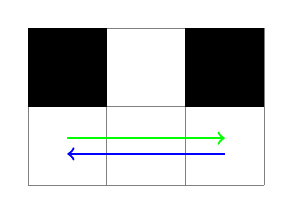
\begin{tikzpicture}
		\draw[step=1cm,gray,very thin] (0,0) grid (3,2);
		\fill[black] (0,1) rectangle ++(1,1);
		\fill[black] (2,1) rectangle ++(1,1);
		\draw[thick,->,color=green] (0.5,0.6) -- (2.5,0.6);
		\draw[thick,<-,color=blue] (0.5,0.4) -- (2.5,0.4);
		\end{tikzpicture}
	\end{figure}
	
	\begin{compactitem}
		\item $a_1assigned: \{1, 2, 3\}$
		\item $a_2assigned: \{3, 2, 1\}$
	\end{compactitem}

	\item \textbf{Check for collisions:} Here we check the MIP path assignment by finding the first collision (if one exists).
	\begin{figure}[H]
		\centering
		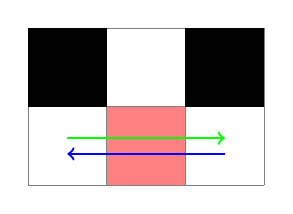
\begin{tikzpicture}
		\draw[step=1cm,gray,very thin] (0,0) grid (3,2);
		\fill[black] (0,1) rectangle ++(1,1);
		\fill[black] (2,1) rectangle ++(1,1);
		\fill[red!50!white] (1,0) rectangle ++(1,1);
		\draw[thick,->,color=green] (0.5,0.6) -- (2.5,0.6);
		\draw[thick,<-,color=blue] (0.5,0.4) -- (2.5,0.4);
		\end{tikzpicture}
	\end{figure}
	
	\begin{compactitem}
		\item $a_1assigned: \{1, \textbf{2}, 3\}$
		\item $a_2assigned: \{3, \textbf{2}, 1\}$
		\item Collision at time 1 on tile (1, 0)
	\end{compactitem}

	\item \textbf{Choose path collision with lowest $\Delta$:}
	\begin{compactitem}
		\item Only one collision to choose from with $\Delta$ of 0: $a_1p_1, a_2p_2$
	\end{compactitem}

	\item \textbf{Find alternative path for agents in collision:}
	\begin{compactitem}
		\item $a_1p_2 : \{1, 1, 2, 3\}$
		\item $a_2p_2 : \{3, 3, 2, 1\}$
	\end{compactitem}
	
	\item \textbf{Create path constraints and apply to the MIP}
	\begin{compactitem}
		\item $Not(a_1p_1, a_2p_2)$
	\end{compactitem}

	% Round 2
	\item \textbf{Path assignment:}
	\begin{figure}[H]
		\centering
		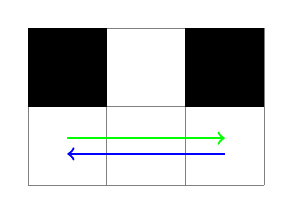
\begin{tikzpicture}
		\draw[step=1cm,gray,very thin] (0,0) grid (3,2);
		\fill[black] (0,1) rectangle ++(1,1);
		\fill[black] (2,1) rectangle ++(1,1);
		\draw[thick,->,color=green] (0.5,0.6) -- (2.5,0.6);
		\draw[thick,<-,color=blue] (0.5,0.4) -- (2.5,0.4);
		\end{tikzpicture}
	\end{figure}
	\begin{compactitem}
		\item $a_1assigned: \{1, 1, 2, 3\}$
		\item $a_2assigned: \{3, 2, 1\}$
	\end{compactitem}

	\item \textbf{Check for collisions:}
	\begin{figure}[H]
		\centering
		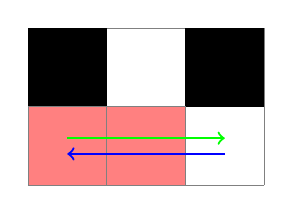
\begin{tikzpicture}
		\draw[step=1cm,gray,very thin] (0,0) grid (3,2);
		\fill[black] (0,1) rectangle ++(1,1);
		\fill[black] (2,1) rectangle ++(1,1);
		\filldraw[red!50!white, draw=gray, very thin] (1,0) rectangle ++(1,1);
		\filldraw[red!50!white, draw=gray, very thin] (0,0) rectangle ++(1,1);
		\draw[thick,->,color=green] (0.5,0.6) -- (2.5,0.6);
		\draw[thick,<-,color=blue] (0.5,0.4) -- (2.5,0.4);
		\end{tikzpicture}
	\end{figure}
	
	\begin{compactitem}
		\item $a_1assigned: \{1, \textbf{1}, \textbf{2}, 3\}$
		\item $a_2assigned: \{3, \textbf{2}, \textbf{1}\}$
		\item Collision at time 2 on tile (1, 0) and tile (0, 0)
	\end{compactitem}

	\item \textbf{Choose path collision with lowest $\Delta$:}
	\begin{compactitem}
		\item Only one collision to choose from with $\Delta$ of 1: $a_1p_1, a_2p_2$
	\end{compactitem}

	\item \textbf{Find alternative path for agents in collision:}
	\begin{compactitem}
		\item $a_1p_2 : \{1, 1, 2, 3\}$
		\item $a_2p_2 : \{3, 2, 2, 1\}$
	\end{compactitem}
	
	\item \textbf{Create path constraints and apply to the MIP}
	\begin{compactitem}
		\item $Not(a_1p_1, a_2p_2)$
	\end{compactitem}

	% Round 3
	\item \textbf{Path assignment:}
	\begin{figure}[H]
		\centering
		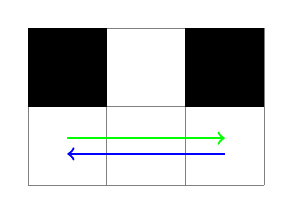
\begin{tikzpicture}
		\draw[step=1cm,gray,very thin] (0,0) grid (3,2);
		\fill[black] (0,1) rectangle ++(1,1);
		\fill[black] (2,1) rectangle ++(1,1);
		\draw[thick,->,color=green] (0.5,0.6) -- (2.5,0.6);
		\draw[thick,<-,color=blue] (0.5,0.4) -- (2.5,0.4);
		\end{tikzpicture}
	\end{figure}
	\begin{compactitem}
		\item $a_1assigned: \{1, 2, 3\}$
		\item $a_2assigned: \{3, 2, 2, 1\}$
	\end{compactitem}
	
	\item \textbf{Check for collisions:}
	\begin{figure}[H]
		\centering
		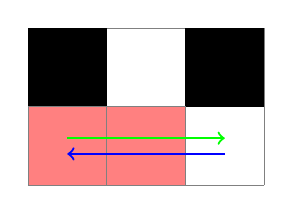
\begin{tikzpicture}
		\draw[step=1cm,gray,very thin] (0,0) grid (3,2);
		\fill[black] (0,1) rectangle ++(1,1);
		\fill[black] (2,1) rectangle ++(1,1);
		\filldraw[red!50!white, draw=gray, very thin] (1,0) rectangle ++(1,1);
		\filldraw[red!50!white, draw=gray, very thin] (0,0) rectangle ++(1,1);
		\draw[thick,->,color=green] (0.5,0.6) -- (2.5,0.6);
		\draw[thick,<-,color=blue] (0.5,0.4) -- (2.5,0.4);
		\end{tikzpicture}
	\end{figure}
	
	\begin{compactitem}
		\item $a_1assigned: \{1, \textbf{2}, 3\}$
		\item $a_2assigned: \{3, \textbf{2}, 2, 1\}$
		\item Collision at time 1 on tile 2
	\end{compactitem}
	
	\item \textbf{Choose path collision with lowest $\Delta$:}
	\begin{compactitem}
		\item Only one collision to choose from with $\Delta$ of 1: $a_1p_1, a_2p_3$
	\end{compactitem}
	
	\item \textbf{Find alternative path for agents in collision:}
	\begin{compactitem}
		\item $a_1p_3 : \{1, 1, 1, 2, 3\}$
		\item $a_2p_3 : \{3, 2, 1, 1\}$
	\end{compactitem}
	
	\item \textbf{Create path constraints and apply to the MIP}
	\begin{compactitem}
		\item $Not(a_1p_1, a_2p_2)$
	\end{compactitem}
	
	\item \textbf{What path / penalty would give the path $\{1, 2, 4, 2, 3\}$?}
	\begin{compactitem}
		\item Penalty on tile 3 timestep 2
		\item Penalty on tile 2 timestep 3
		\item Hence the path would look like: $\{3, 3, 3, 2, 1\}$
	\end{compactitem}

	\item \textbf{What path / penalty would give the path $\{3, 3, 3, 2, 1\}$?}
	\begin{compactitem}
		\item Penalty on tile 2 timestep 2
		\item Penalty on tile 2 timestep 3
		\item Hence the path would look like: $\{1, 2, 2, 3\}$
	\end{compactitem}
	
\end{enumerate}




\bibliographystyle{dcu}
\bibliography{bibliography}
	
\end{document}
